\section{Simulation Details and the Jet Image}
\label{sec:simulation}

In order to study jet images in a realistic scenario, we use Monte Carlo (MC) simulations of high energy particle collisions. One important jet tagging application is the identification of highly Lorentz boosted $W$ bosons decaying into quarks amidst a large background from the generic production of quarks and gluons.  This classification task has been thoroughly studied experimentally\footnote{There is also an extensive literature on phenomenological studies - see references within the experimental papers.}~\cite{Khachatryan:2014vla,ATL-PHYS-PUB-2015-033,ATL-PHYS-PUB-2014-004} and used in many analyses~\cite{Aad:2015owa,Khachatryan:2014hpa,Khachatryan:2015mta,Khachatryan:2015oba,Khachatryan:2015gza,Khachatryan:2015bma,Khachatryan:2015cwa,Khachatryan:2015ywa,Aad:2014wea,Aad:2015agg,Aad:2015kna,Aad:2015ufa,Aad:2014haa}.  

To simulate highly boosted $W$ bosons, a hypothetical $W'$ boson is generated and forced to decay to a hadronically decaying $W$ boson ($W\rightarrow qq'$) and a $Z$ boson which decays invisibly ($Z\rightarrow \nu\bar{\nu}$).  The mass of the $W'$ boson determines the Lorentz boost of the $W$ boson in the lab frame since the $W'$ is produced nearly at rest and the $W$ boson momentum is approximately $m_{W'}/2$.  The invisible decay of the $Z$ boson ensures that the jet in the event with the highest transverse momentum is the $W$ boson jet.  Multijet production of quarks and gluons is simulated as a background.  Both the $W'$ signal and the multijet background are generated using \textsc{Pythia} 8.170~\cite{Pythia8,Pythia} at $\sqrt{s}=14$ TeV.  The angular separation of the $W$ boson decay products in the plane transverse to the beam direction scales as $2m_{W}/p_{T,W}$, where $m_W\approx 80$~GeV and $p_{T,W}$ is the component of the $W$ boson momentum in this plane.  The tagging strategy and performance depend strongly on $p_{T,W}$, so we focus on a particular range: $250$~GeV~$<p_{T,W}<300$~GeV.  This corresponds to an angular spread of about $1$ radian.  The decay products of the $W$ bosons as well as the background are clustered into jets using the anti-$k_t$ algorithm~\cite{antiktpaper} via \textsc{FastJet}~\cite{fastjet} 3.0.3.  To mitigate the contribution from the underlying event, jets are are trimmed~\cite{trimming} by re-clustering the constituents into $R=0.3$ $k_t$ subjets and dropping those which have $p_T^\text{subjet}<0.05\times p_T^\text{jet}$. 

To model the discretization and finite acceptance of a real detector, a calorimeter of towers with size $0.1\times 0.1$ in $(\eta,\phi)$ extends out to $\eta=5.0$.  The total energy of the simulated particles incident upon a particular cell are added as scalars and the four-vector $p_j$ of any particular tower $j$ is given by

\begin{align}
\label{eq:calo}
p_j = \sum_{i\text{ incident on $j$}}E_i(\cos\phi_j/\cosh \eta_j,\sin\phi_j/\cosh \eta_j,\sinh \eta_j/\cosh \eta_j,1),
\end{align}

\noindent where $E_i$ is the energy of particle $i$ and the center of the tower $j$ is $(\eta_j,\phi_j)$.  Towers are treated as massless.

 A {\it jet image} is formed by taking the constituents of a jet and discretizing its energy into pixels in ($\eta,\phi$), with the intensity of each pixel given by the sum of the energy of all constituents of the jet inside that ($\eta,\phi$) pixel.  In our studies, we take the jet image pixelation to match the simulated calorimeter tower granularity.  In the next section, we will discuss the nuances of standardizing the coordinates of a jet image as a pre-processing step prior to applying machine learning.  
 
pT weighting

\begin{figure}[bt]
  \begin{center}
        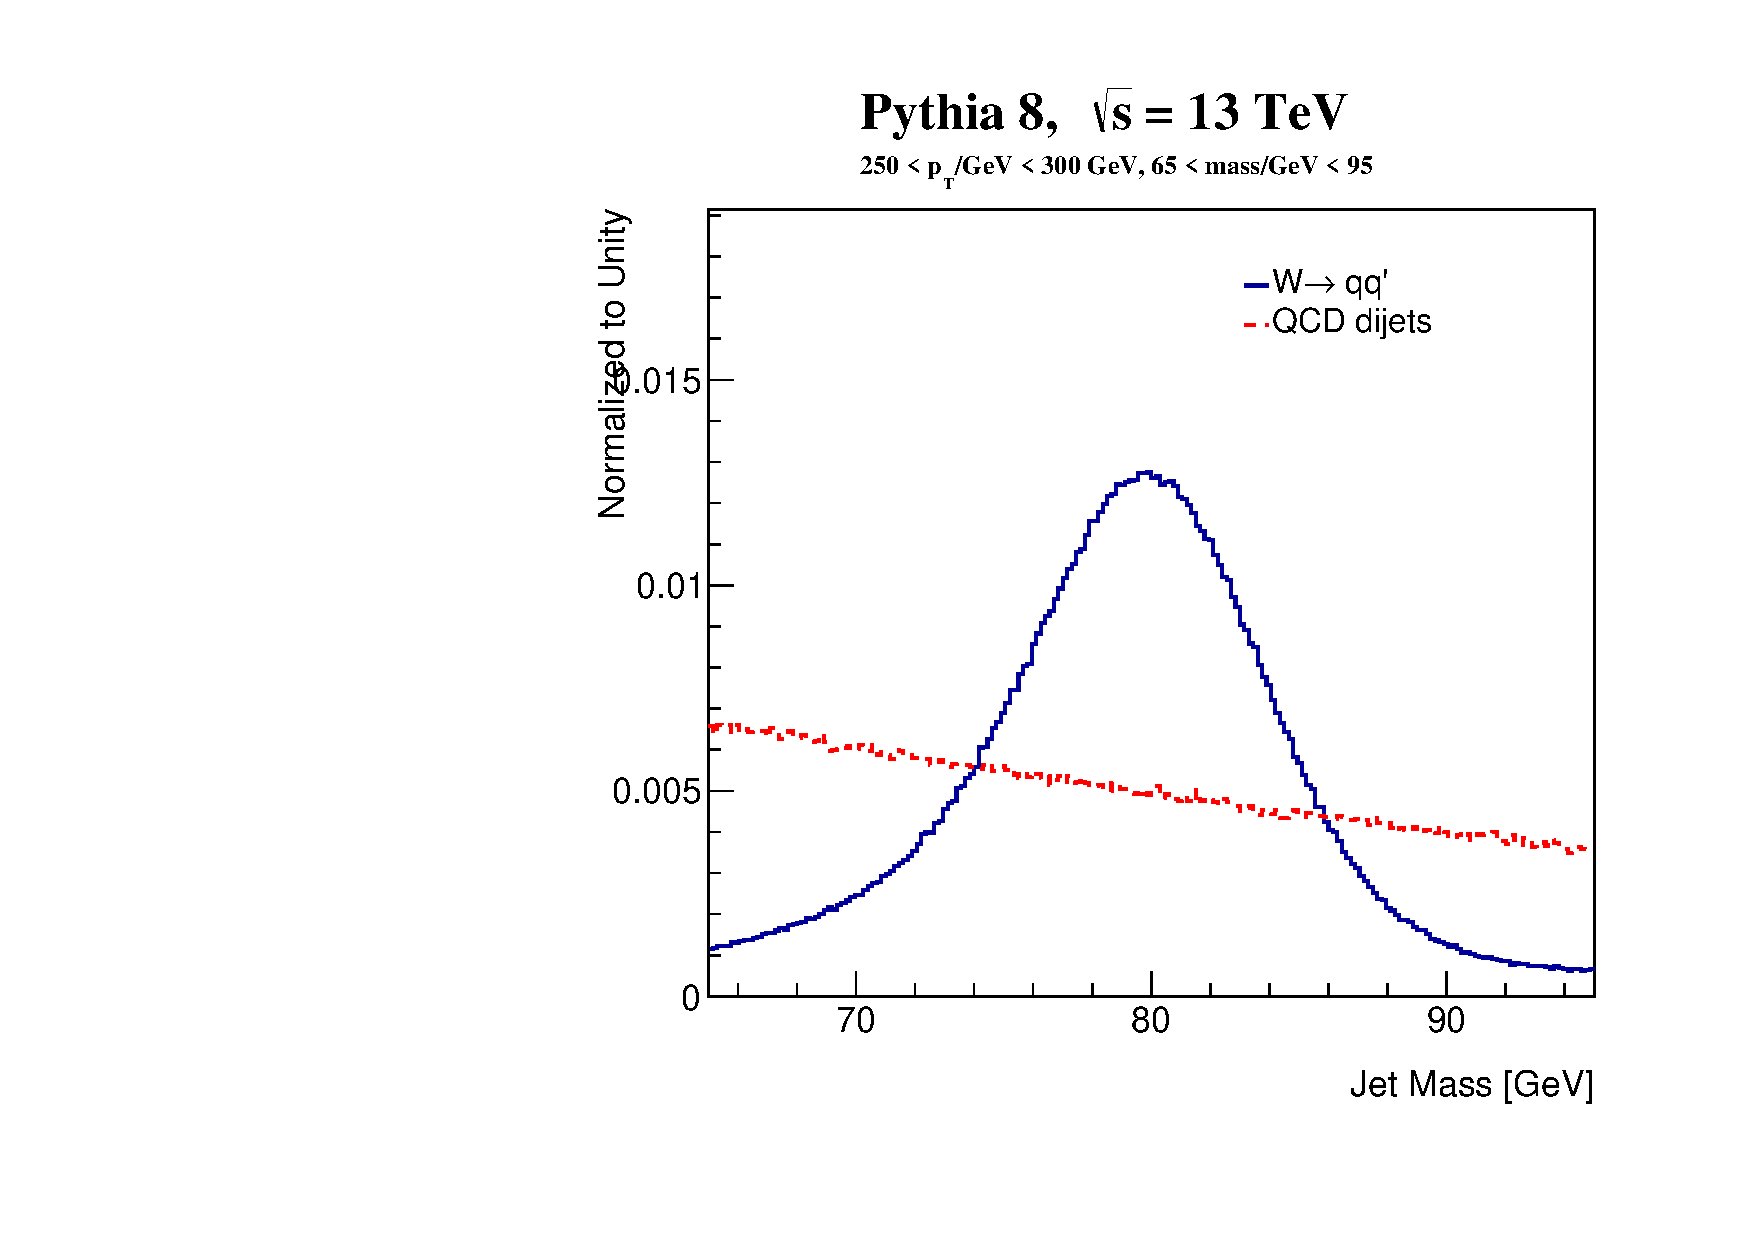
\includegraphics[width=0.45\textwidth]{figures/mass.pdf} 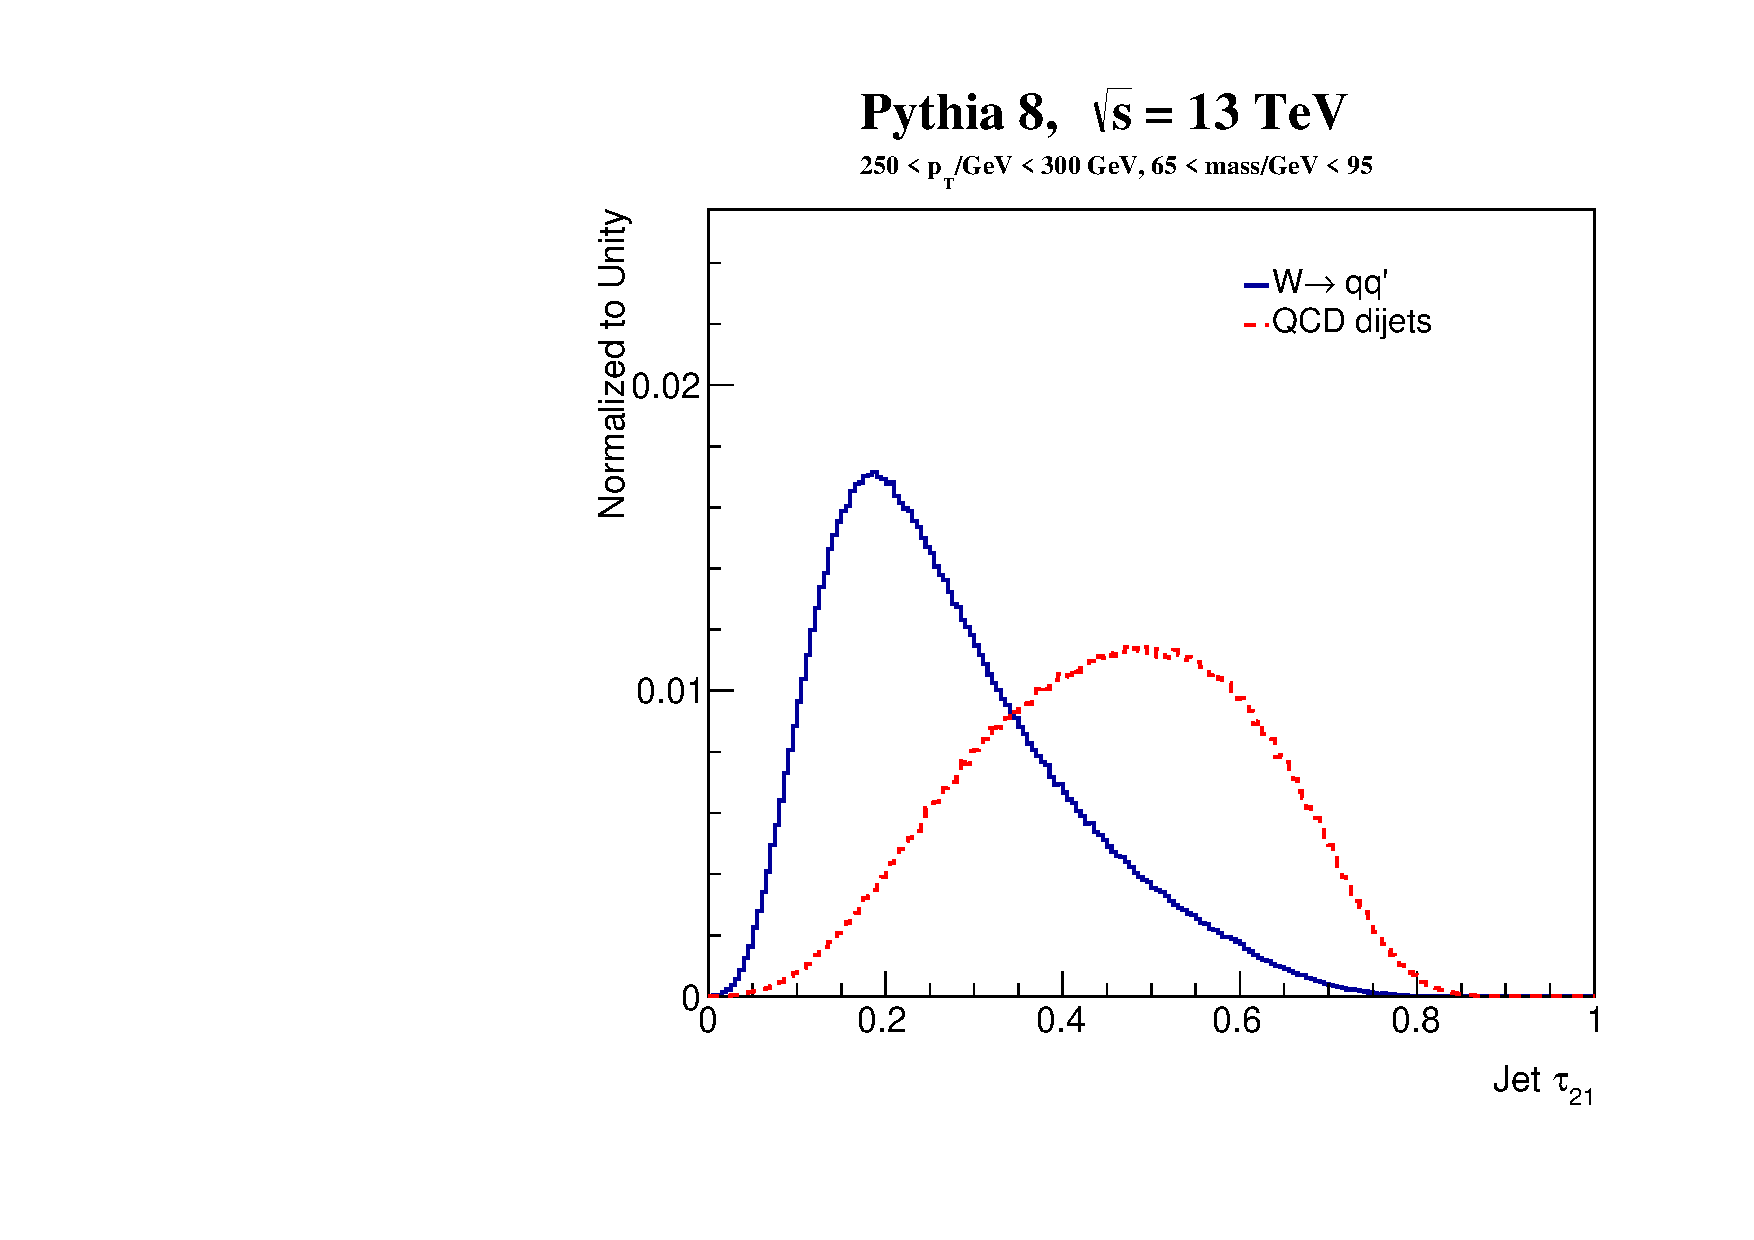
\includegraphics[width=0.45\textwidth]{figures/tau21.pdf} \\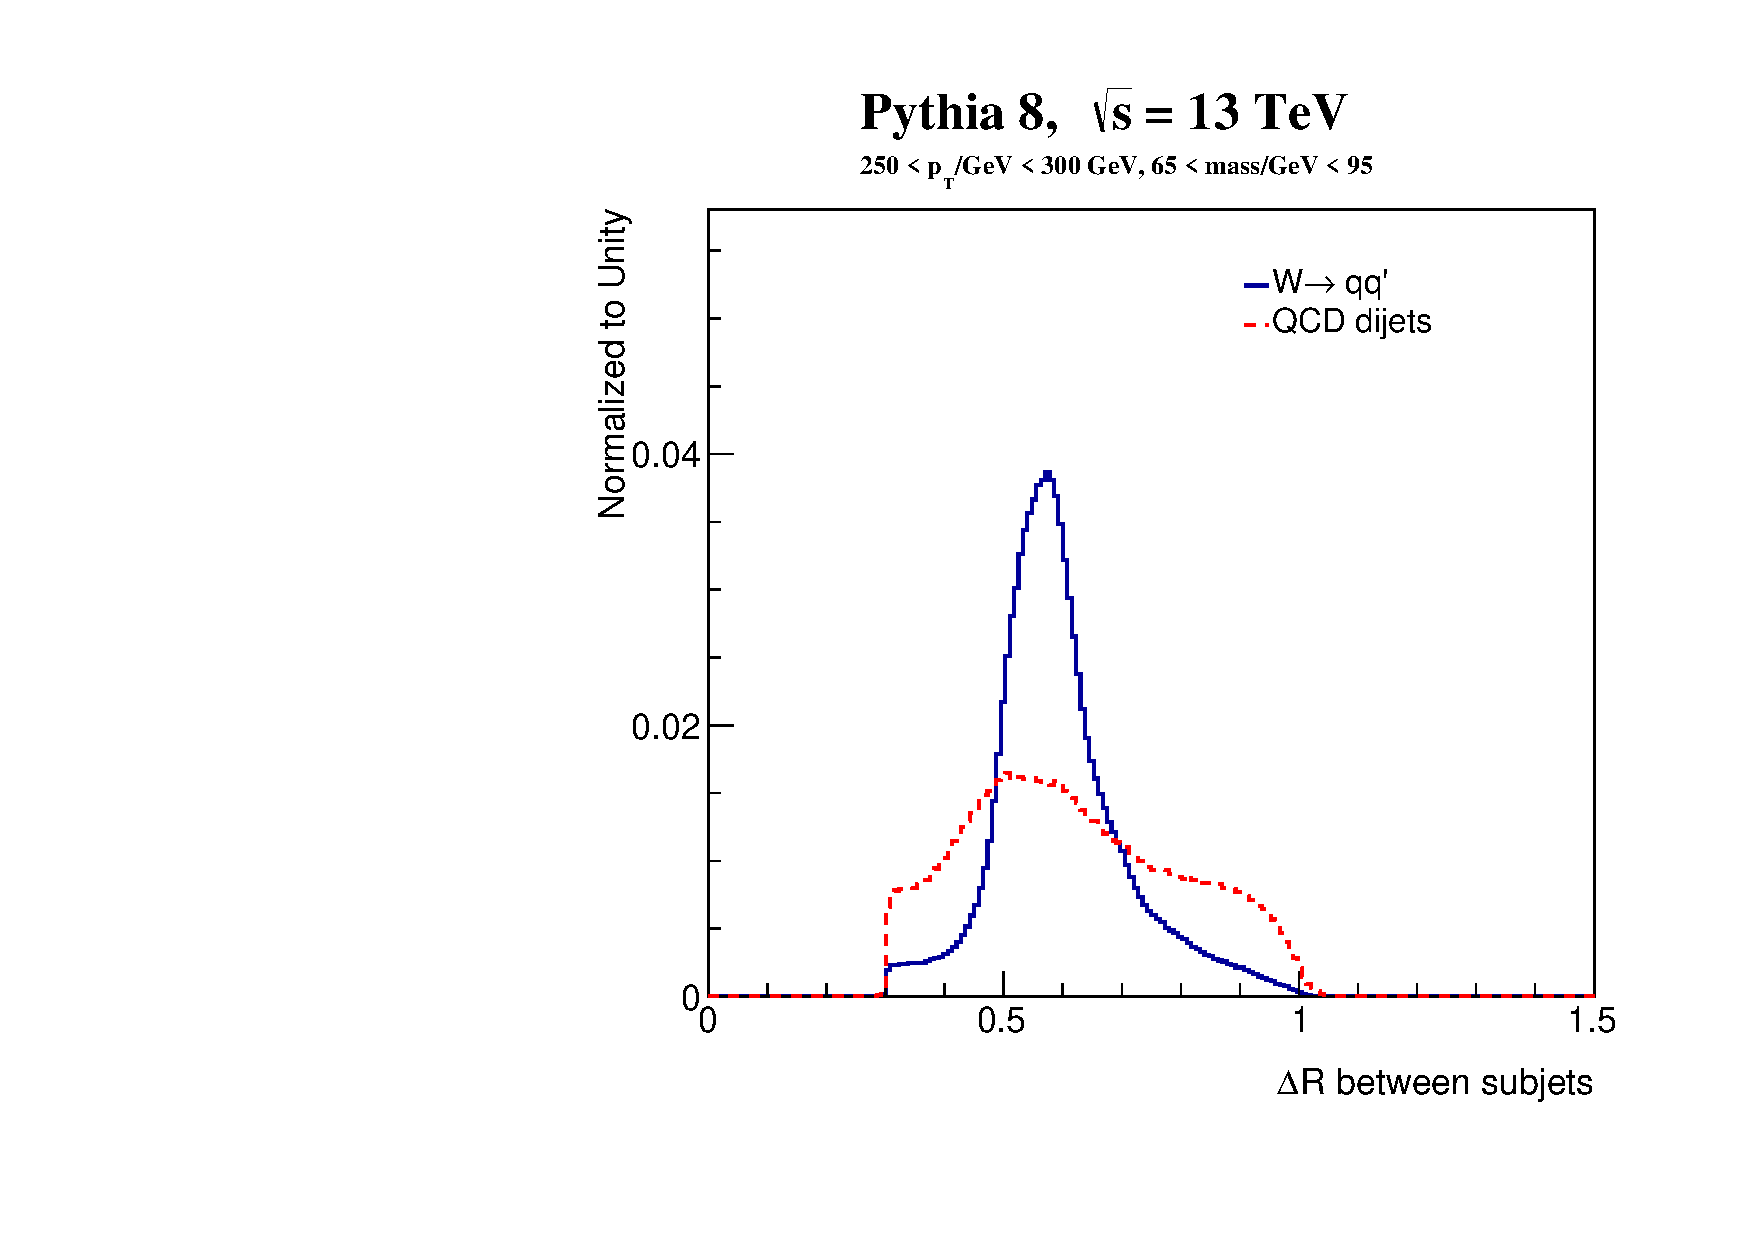
\includegraphics[width=0.45\textwidth]{figures/dR.pdf}
      \caption{ 
      \label{fig:datastats} }
    \end{center}
\end{figure}

\newpage
\clearpage

\section{Pre-processing and the Symmetries of Space-time}
\label{sec:preprocess}

In order for the machine learning algorithms to most efficiency learn discriminating features between signal and background and not learn the symmetries of space-time, the jet images are pre-processed.  This procedure can greatly improve performance and reduce the required size of the sample used for testing.  Our pre-processing procedure happens in four steps: translation, rotation, re-pixelation, and inversion.  To begin, the jet images are translated so that the leading subjet is at $(\eta,phi)=(0,0)$.  Translations in $\phi$ are rotations around the $z$-axis and so the pixel intensity is unchanged by this operation.  On the other hand, translations in $\eta$ are {\it Lorentz boosts} along $z$, which do not preserve the pixel intensity.  Therefore, a proper translation in $\eta$ would modify the pixel intensity.  One simple modification of the jet image to circumvent this change is to replace the pixel intensity $E_i$ with $p_{T,i}=E_i/\cosh(\eta_i)$.  This new definition of intensity is invariant under translations in $\eta$ and is used exclusively for the rest of this paper.

The second step of pre-processing is to rotate the images around the center of the jet.  If a jet has a second subjet, then the rotation is performed so that the second subjet is at $-\pi/2$.  If no second subjet exists, then the jet image is rotated so that the first principle component of the pixel intensity distribution is at $-\pi/2$.  Unless the rotation is by an integer multiple of $\pi/4$, the rotated grid will not line up with the original grid.  Therefore, the energy in the rotated grid must be re-distributed amongst the pixels of the original image grid.  A cublic spline interpolation is used in this case - see Ref.~\cite{Cogan:2014oua} for details.  The last step is a parity flip so that the right side of the jet image has the highest sum pixel intensity.  

Figure~\ref{fig:preprocess} shows the average jet image for $W$ boson jets and QCD jets before and after the rotation, re-pixelation, and inversion steps of the pre-processing.  The more pronounced second-subjet is already pronounced in the left plots of Fig.~\ref{fig:preprocess}, where there is a clear annulus for the signal $W$ jets which is nearly absent for the background QCD jets.  However, after the rotation, the second core of energy is well isolated and localized in the images.  The spread of energy around the leading subjet is more diffuse for the QCD background which consists largely of gluon jets which have an octet radiation pattern compared to the singlet radiation pattern of the $W$ jets, where the radiation is mostly restricted to the region between the two hard cores.

\begin{figure}[bt]
  \begin{center}
        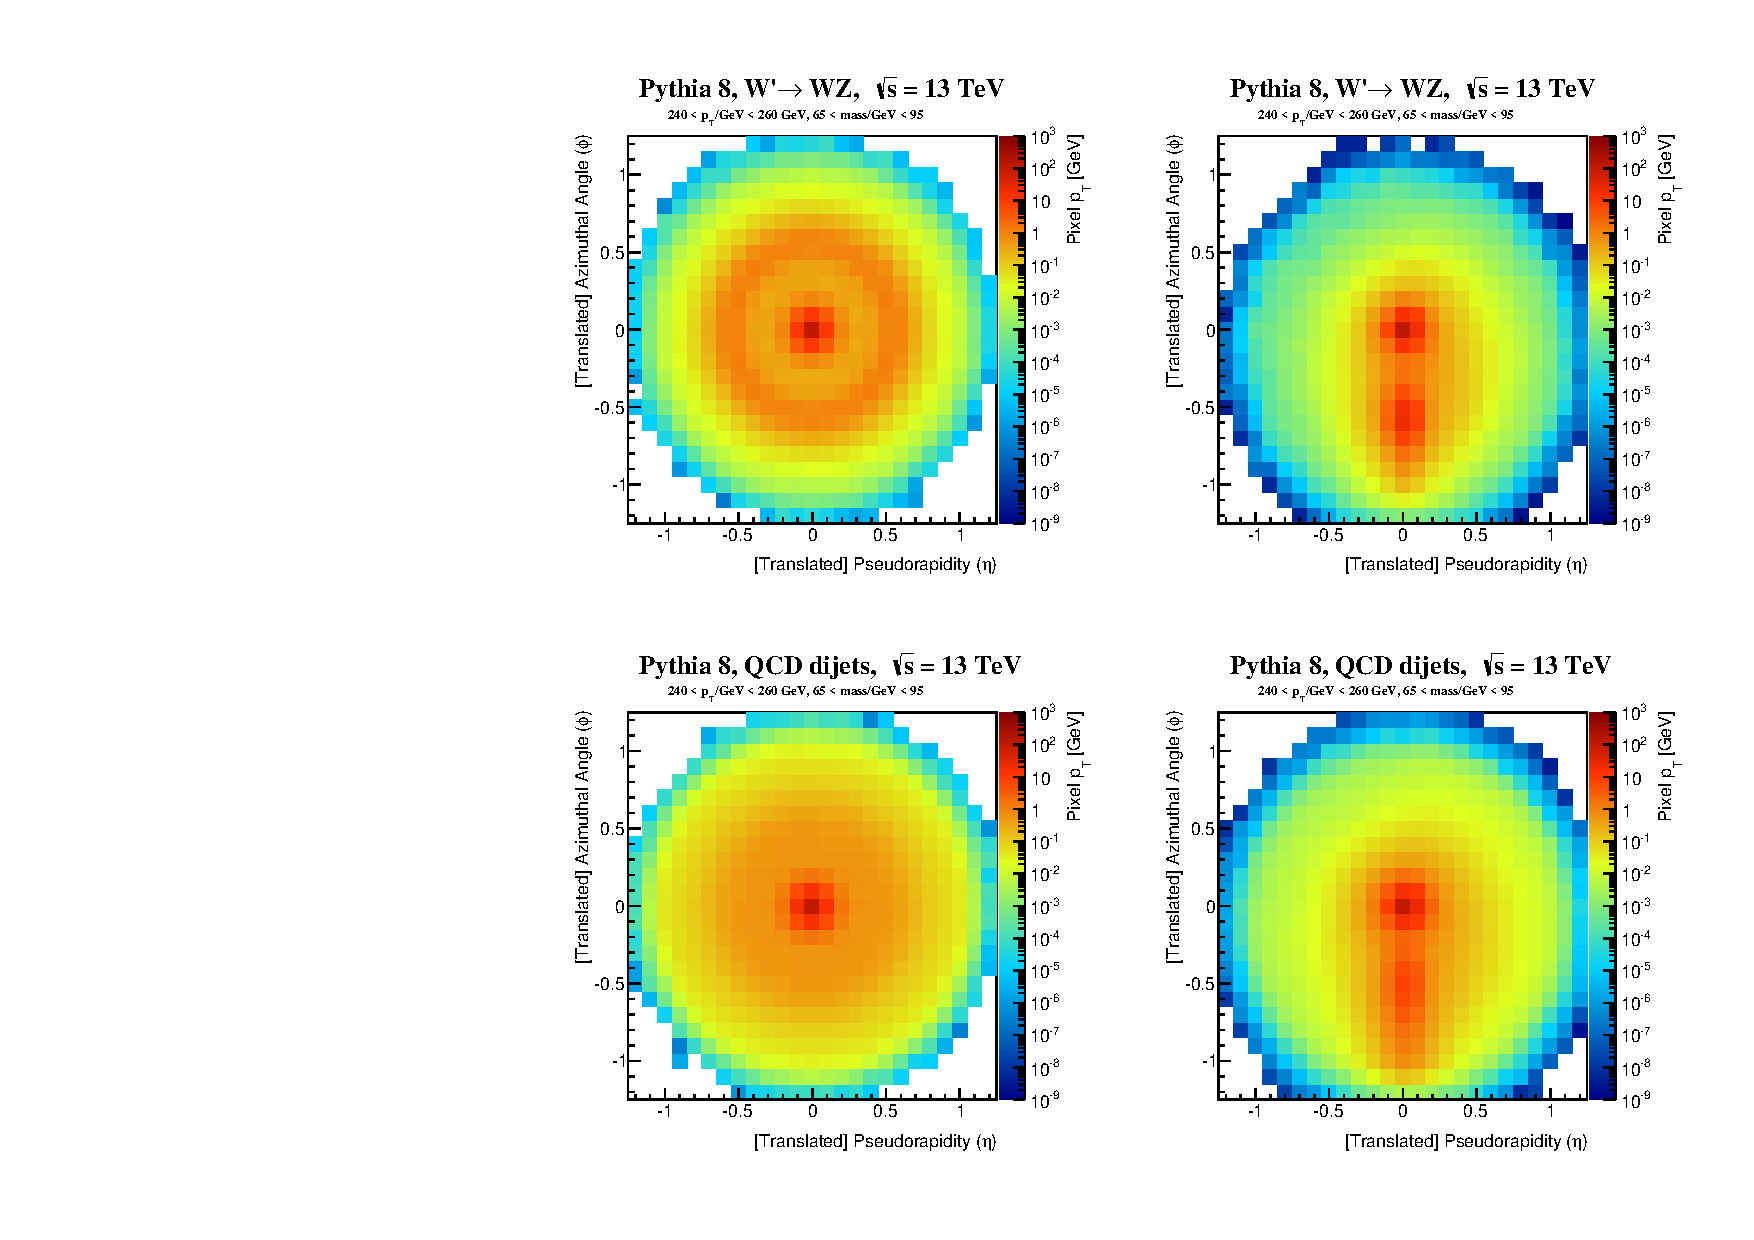
\includegraphics[width=0.99\textwidth]{figures/Image_mass_average_fixed_nonorm.pdf}
      \caption{ The average jet image for signal $W$ jets (top) and background QCD jets (bottom) before (left) and after (right) applying the rotation, re-pixelation, and inversion steps of the pre-processing.  The average is taken over images of jets with $240$ GeV $<p_T<$ 260 GeV and 65~GeV~$<$ mass $<$~95~GeV.
      \label{fig:preprocess} }
    \end{center}
\end{figure}

One standard pre-processing step that is often additionally applied in machine learning is normalization.  A common normalization scheme is the $L^2$ norm such that $\sum I_i^2=1$ where $I_i$ is the intensity of pixel $i$.  This is particularly useful for the jet images where pixel intensities can span many orders of magnitude.  The jet transverse momenta are all around 250 GeV, but this can be spread amongst many pixels or concentrated in only a few and the $L^2$ norm helps mitigate the spread and thus makes training easier for the machine learning algorithm.  However, normalization can distort information contained within the jet image.  Some information, such as the Euclidean distance $\Delta R$ between subjets in $(\eta,\phi)$ is invariant under all of the pre-processing steps as well as normalization.  However, consider the {\it image mass}, 

\begin{align}
m_I^2=\sum_{i<j} E_iE_j(1-\cos(\theta_{ij})),
\end{align}

\noindent where $E_i=I_i/cosh(\eta_i)$ for pixel intensity $I_i$ and $\theta_{ij}$ is the angle between massless four-vectors with $\eta$ and $\phi$ at the $i$ and $j$ pixel centers.  The image mass is not invariant under all pre-processing steps, but does encode useful discrimination information.  As discussed earlier, with the proper choice of pixel intensity, translations preserve the image mass since it is a Lorentz invariant quantity.  However, the rotation pre-processing step does not preserve the image mass.  To see this, consider two four-vectors: $p^\mu=(1,0,0,1)$ and $q^\mu=(0,1,0,1)$.   The invariant mass of these vectors is $\sqrt{2}$.  The vector $p^\mu$ is at the center of the jet image coordinates and the vector $q^\mu$ is located at $\pi/2$ degrees.  If we rotate the image around the jet axis so that the vector $q^\mu$ is at $0$, akin to rotating the jet image so that the sub-leading subjet goes from $\pi/2$ to $0$, then $p^\mu$ is unchanged but $q^\mu\rightarrow (1,0,\sinh(1),\cosh(1))$.  The new invariant mass of $q^\mu$ and $p^\mu$ is about 1, which is reduced from its original value of $\sqrt{2}$.  The parity inversion pre-processing step does not impact the image mass, but a $I^2$ normalization does modify the image mass.  The easiest way to see this is to take a series of images with exactly the same image mass but variable $I^2$ norm.  The map $I_i\mapsto I_i/\sum_j I_j^2$ modifies the mass by $m_I\mapsto m_I/\sum_j I_j^2$ and so the spread in the normalizations induces a spread in the mass distribution.

The impact of the various stages of pre-processing on the image mass are illustrated in Fig.~\ref{fig:preprocess2}.  The finite granularity of the simulated detector slightly degrades the resolution, but the translation and parity inversion (flip) have no impact, by construction.  The rotation that will have the biggest potential impact on the image mass is by $\pi/2$ (maximally changing $\eta$ and $\phi$), which does lead to a small change in the mass distribution.  A naive translation in $\eta$ that uses the tower energy as the intensity instead of the transverse momentum or an $I^2$ normalization scheme both significantly broaden the mass distribution.  One way to quantify the amount of information in the jet mass that is lost by various pre-processing steps is shown in the Receiver Operator Characteristic (ROC) curve of Fig.~\ref{fig:preprocess3}.   Information about the mass is lost when the ability to use the mass to differentiate signal and background is diminished.  The naive translation and the $I^2$ normalization schemes are significantly worse than the other image mass curves which are themselves similar in performance. 

\begin{figure}[bt]
  \begin{center}
        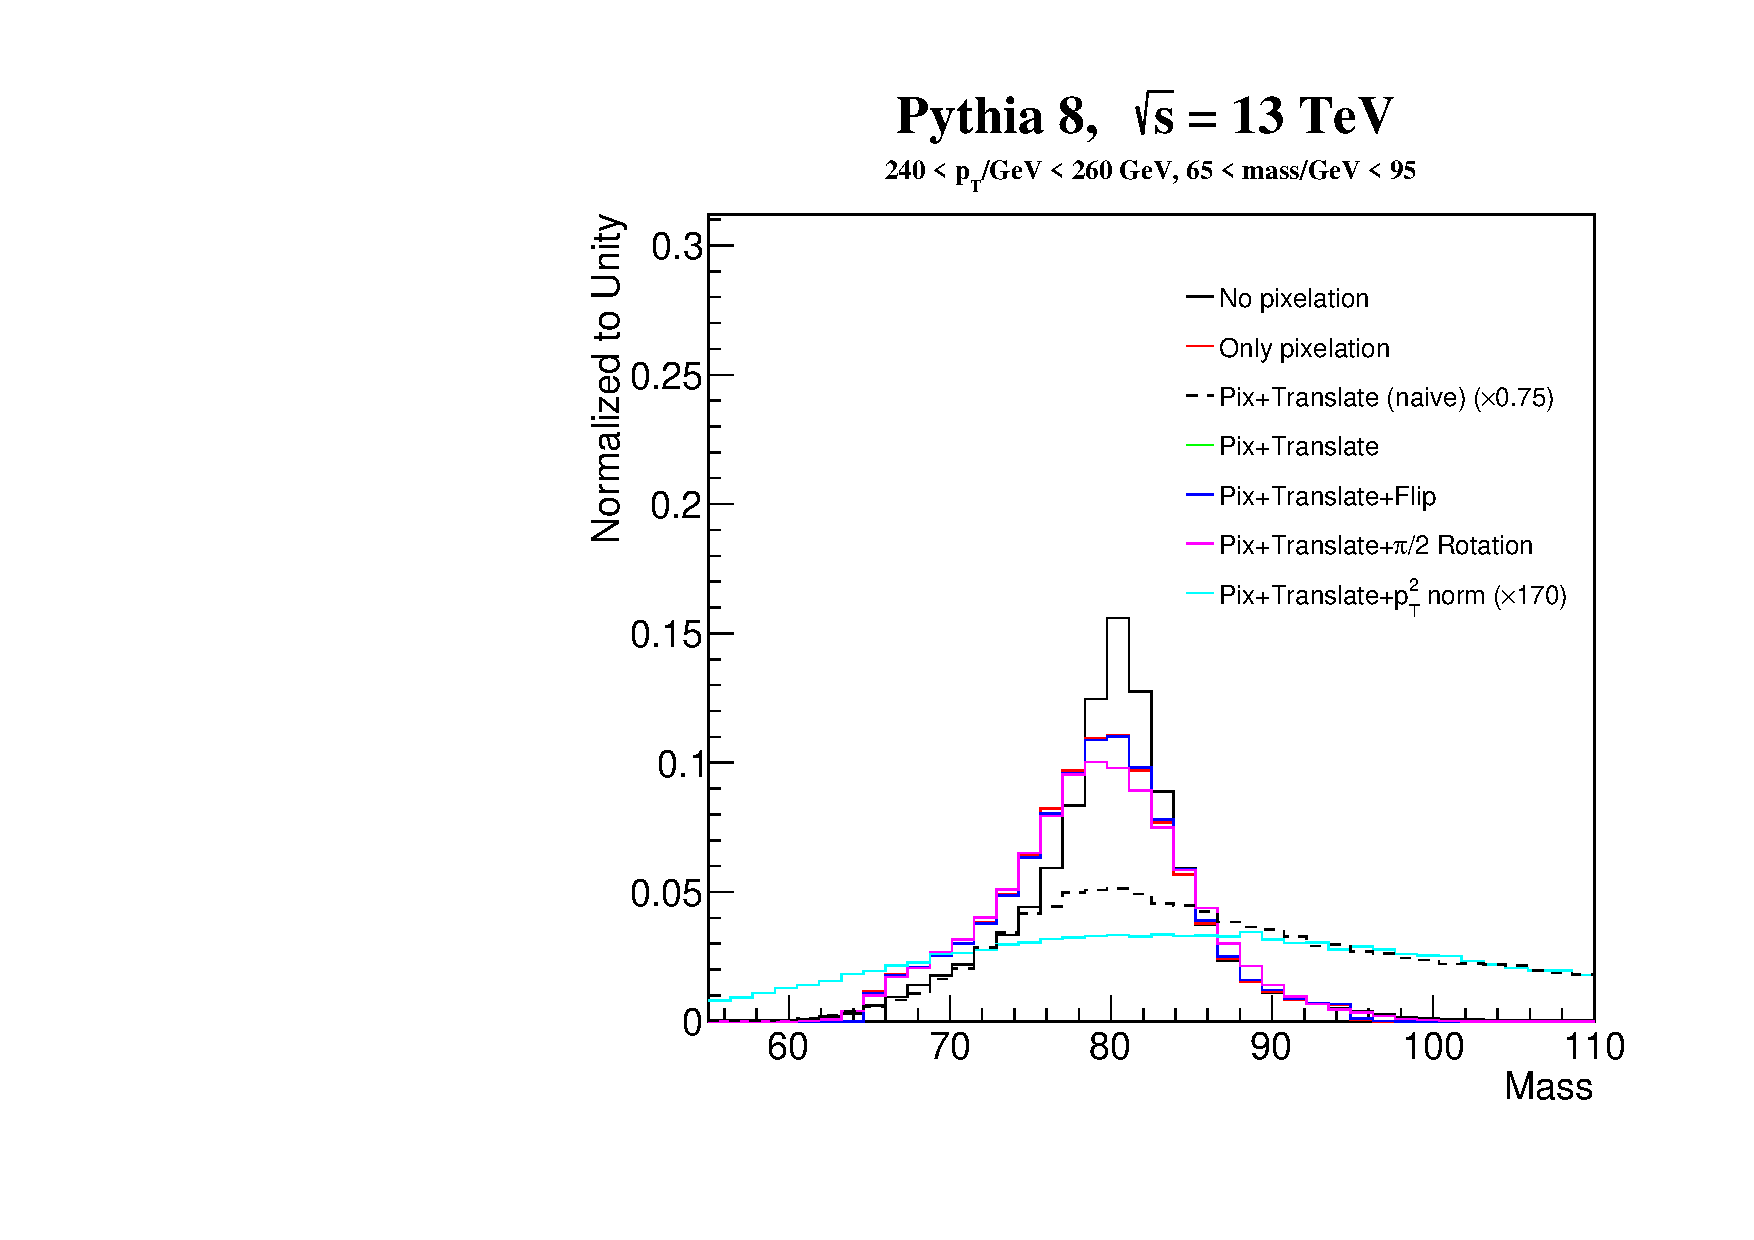
\includegraphics[width=0.5\textwidth]{figures/ImageMass_Comparison.pdf}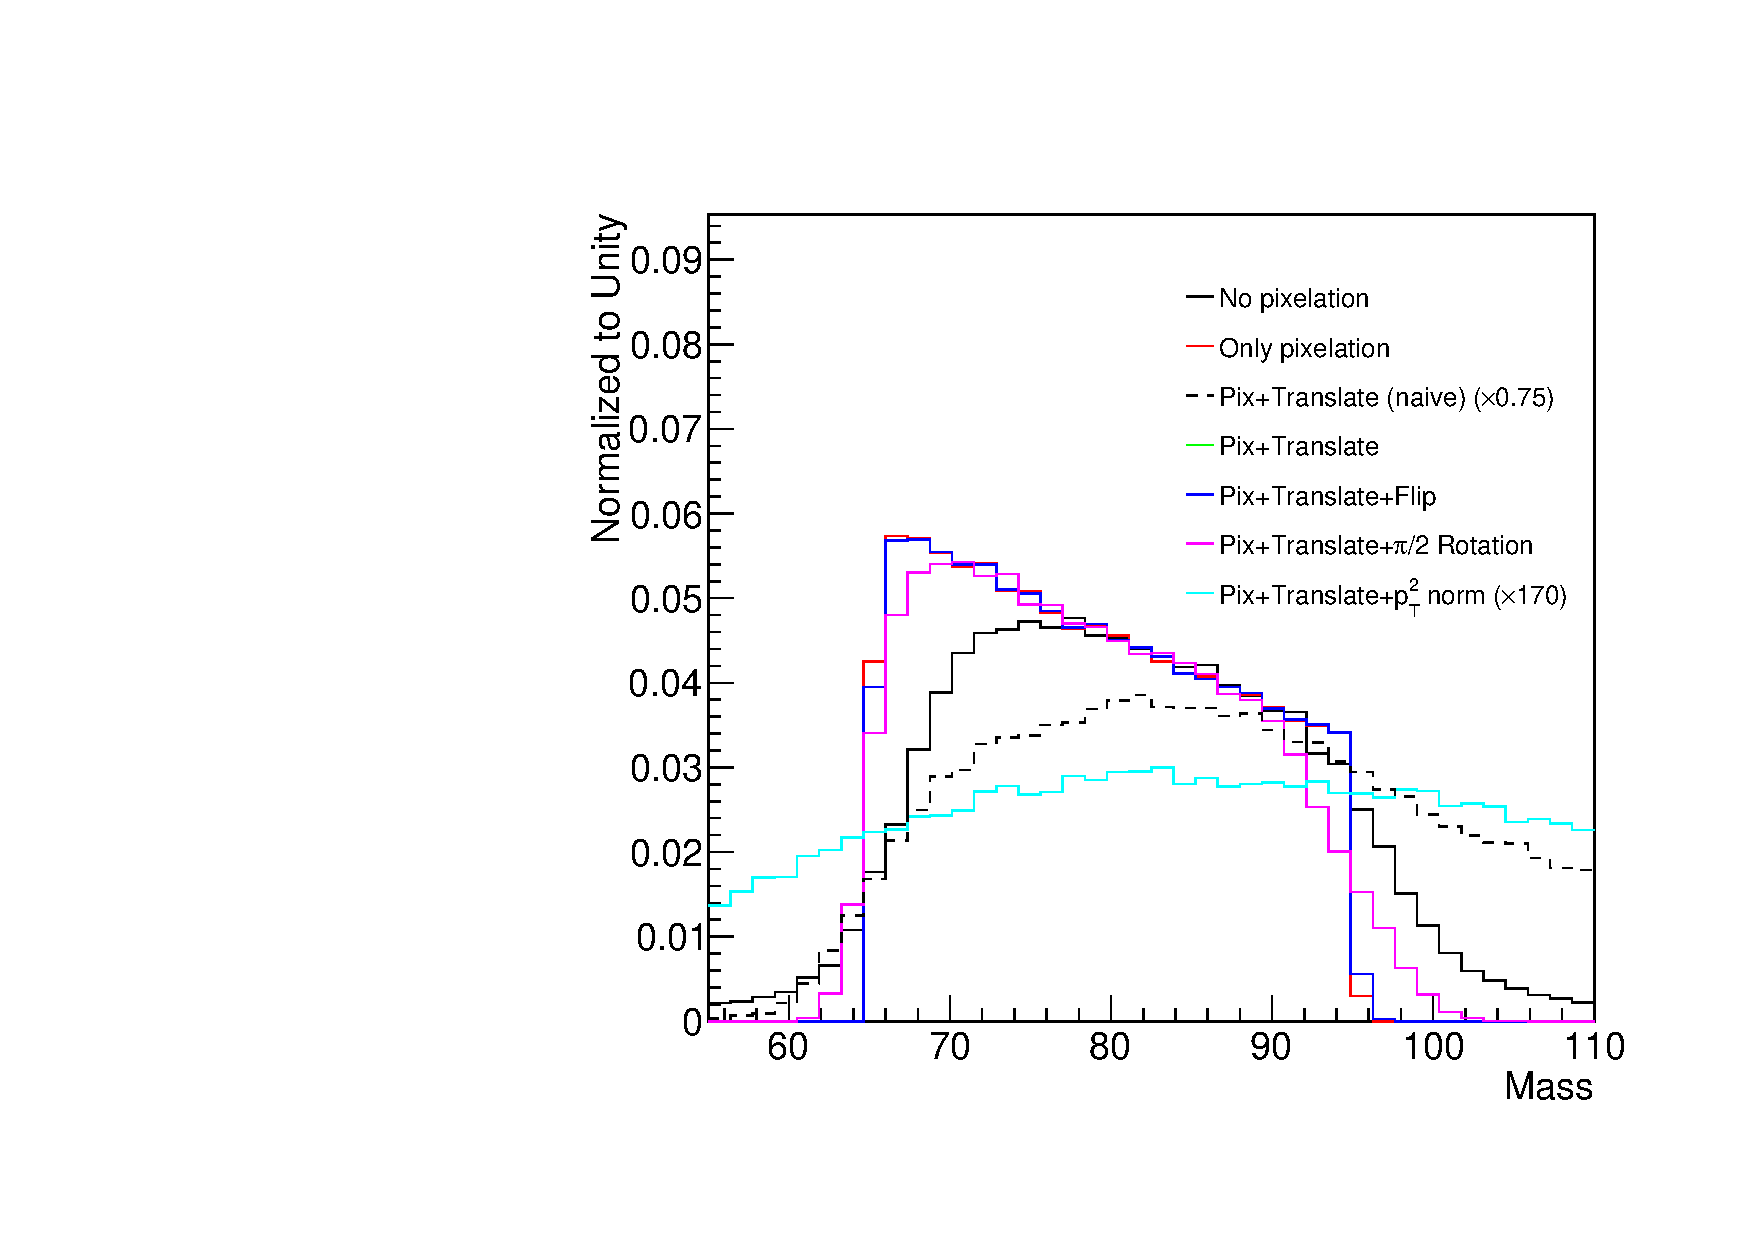
\includegraphics[width=0.5\textwidth]{figures/ImageMass_Comparison_back.pdf}
      \caption{ The distribution of the image mass after various states of pre-processing for signal jets (left) and background jets (right).  The {\it No pixelation line} is the jet mass without any detector granularity and without any pre-processing.  {\it Only pixelation} has only detector granularity but no pre-processing and all subsequent lines have this pixelation applied as well as translation to center the image at the origin.  The translation is called {\it naive} when the energy is used as the pixel intensity instead of the tower transverse momentum.  {\it Flip} denotes the parity inversion operation and the $p_T^2$ norm is a $I^2$ normalization scheme.  The naive translation and the $I^2$ normalization image masses are both multiplied by constants so that the centers of the distribution are roughly in the same location as for the other distributions.
      \label{fig:preprocess2} }
    \end{center}
\end{figure}


\begin{figure}[bt]
  \begin{center}
        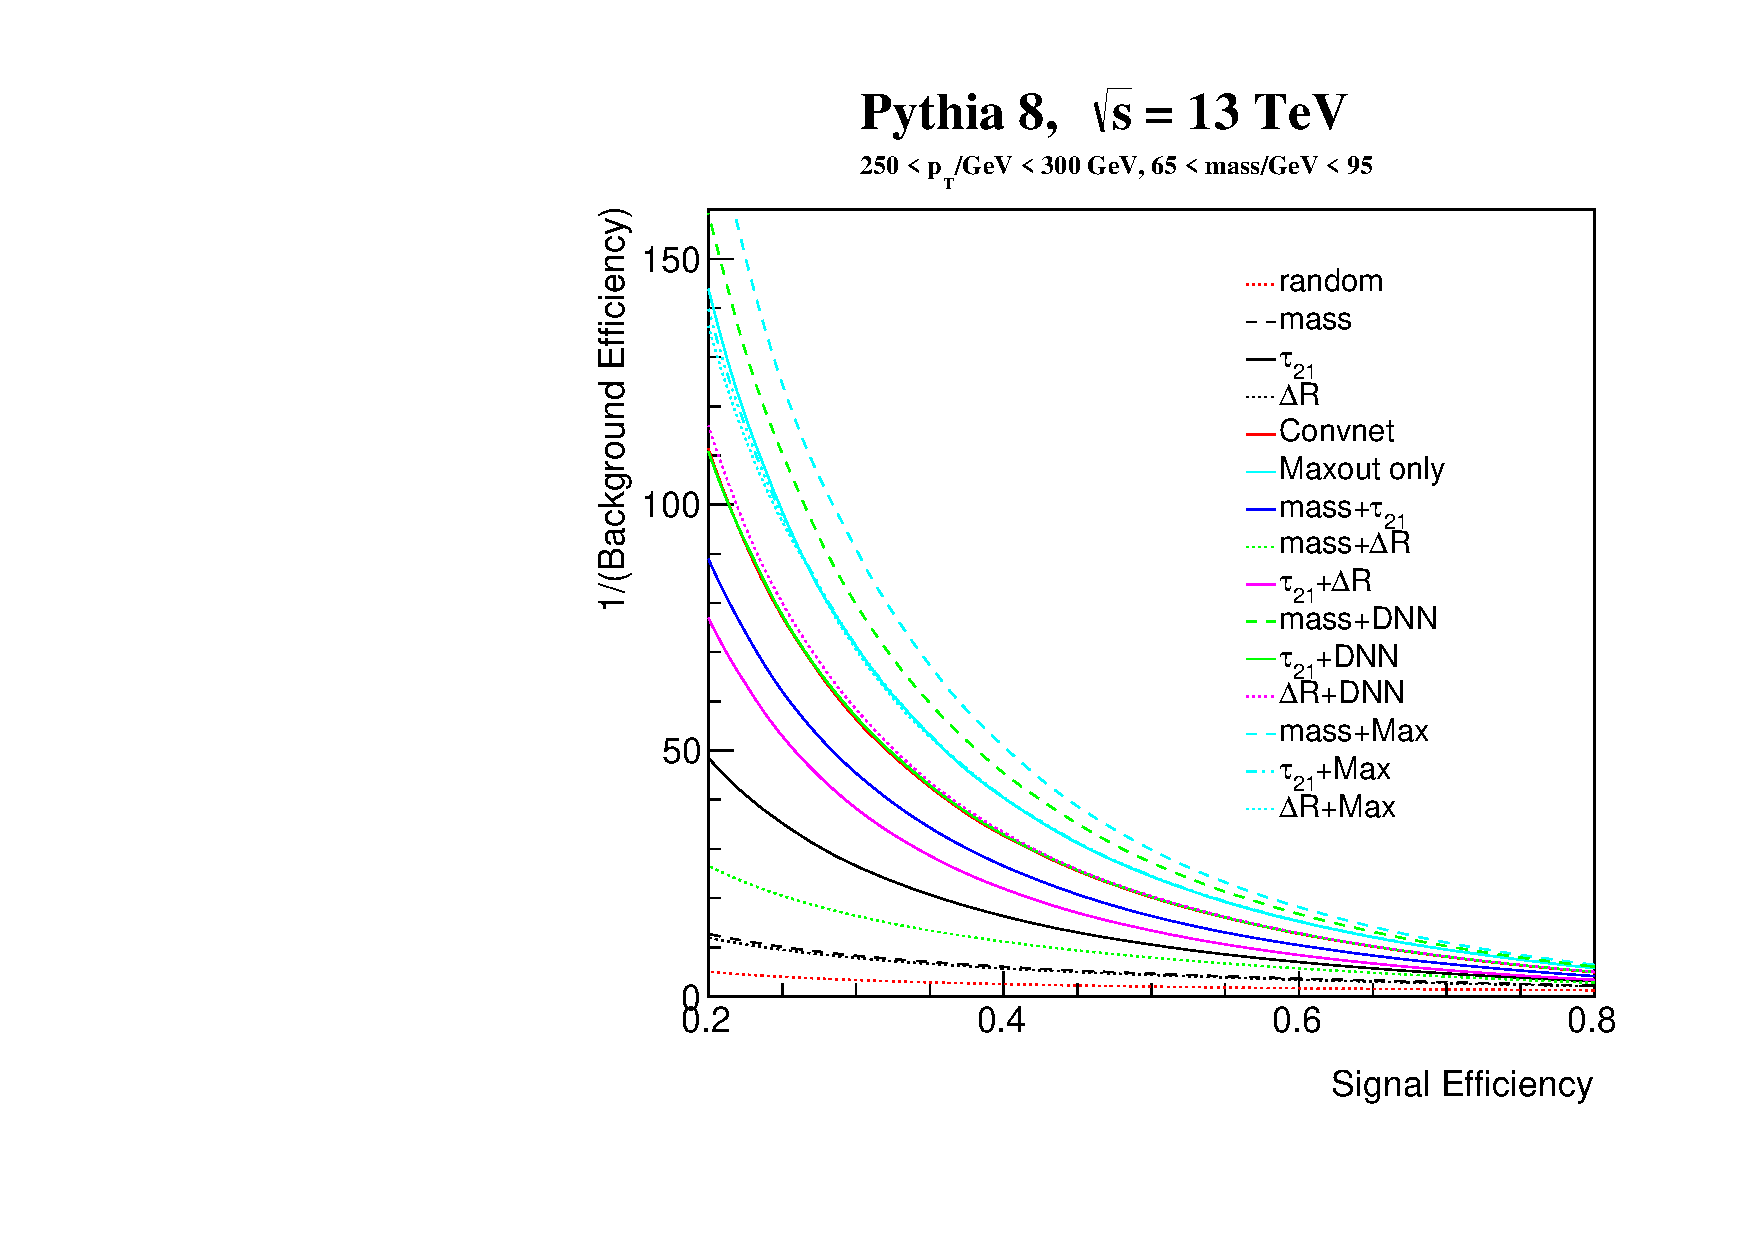
\includegraphics[width=0.99\textwidth]{figures/ROCs.pdf}
      \caption{ The tradeoff between $W$ boson (signal) jet efficiency and inverse QCD (background) efficiency for various pre-processing algorithms applied to the jet (images).  The {\it No pixelation line} is the jet mass without any detector granularity and without any pre-processing.  {\it Only pixelation} has only detector granularity but no pre-processing and all subsequent lines have this pixelation applied as well as translation to center the image at the origin.  The translation is called {\it naive} when the energy is used as the pixel intensity instead of the tower transverse momentum.  {\it Flip} denotes the parity inversion operation and the $p_T^2$ norm is a $I^2$ normalization scheme.  
      \label{fig:preprocess3} }
    \end{center}
\end{figure}

\clearpage
\newpage

